% !TEX root = ../main.tex


%---------------------------------------------------------------------
% 附录
\clearpage
\section{附录}
\vspace{-0.7cm} % 负值缩小间距
\noindent\textcolor{fgraygreen}{\rule{0.382\textwidth}{2pt} }
\vspace{7pt}

\subsection{补充材料}

所有相关材料可以在Github库 \href{https://github.com/TaLEsCuber/CoLabR}{TaLEsCuber/CoLabR} 中找到。

\subsection{实验仪器}

\begin{table}[h]
	\centering
	\caption{热噪声测（玻尔兹曼常量）量仪器用具}
	\resizebox{\textwidth}{!}{\begin{tabular}{ccccc}
		\hline
		\rowcolor{fgraygreen} \textbf{编号} & \textbf{仪器用具名称} & \textbf{数量} & \textbf{主要参数（型号、规格等）} & \textbf{备注} \\ \hline
		1 & 锁相放大器 & 1 & OE1022 & \\ 
		2 & 示波器 & 1 & RIGOL DS2202A & \\ 
		3 & 数字多用表 & 1 & RIGOL DM3058E、MS6514 & \\ 
		4 & 测温仪 & 1 & MS6514 & \\ 
		5 & PC 机 & 1 & LabVIEW 环境及有 VISA 接口协议 & \\ 
		6 & 可变温样品盒（带 BNC 接头） & 1 & 6.6k$\Omega$、13k$\Omega$、41k$\Omega$、66k$\Omega$、98k$\Omega$、144k$\Omega$ & 任选其一 \\ \hline
	\end{tabular}
}
\end{table}

\subsection{原始数据}

\subsection{个人签名}

% 专业、年级、姓名、学号、实验名（或编号）和日期
\infoPersonal{物理学强基计划}{2022级}{杨舒云}{22344020}{APL1-1-A}{2024年10月25日}

\begin{figure}[htbp]
	\centering
	
\includegraphics[width=0.7\textwidth]{name.png}
	\caption{个人签名：杨舒云}
	\label{fig:name}
\end{figure}

\subsection{附表}

\begin{figure}[h!]
	\centering
	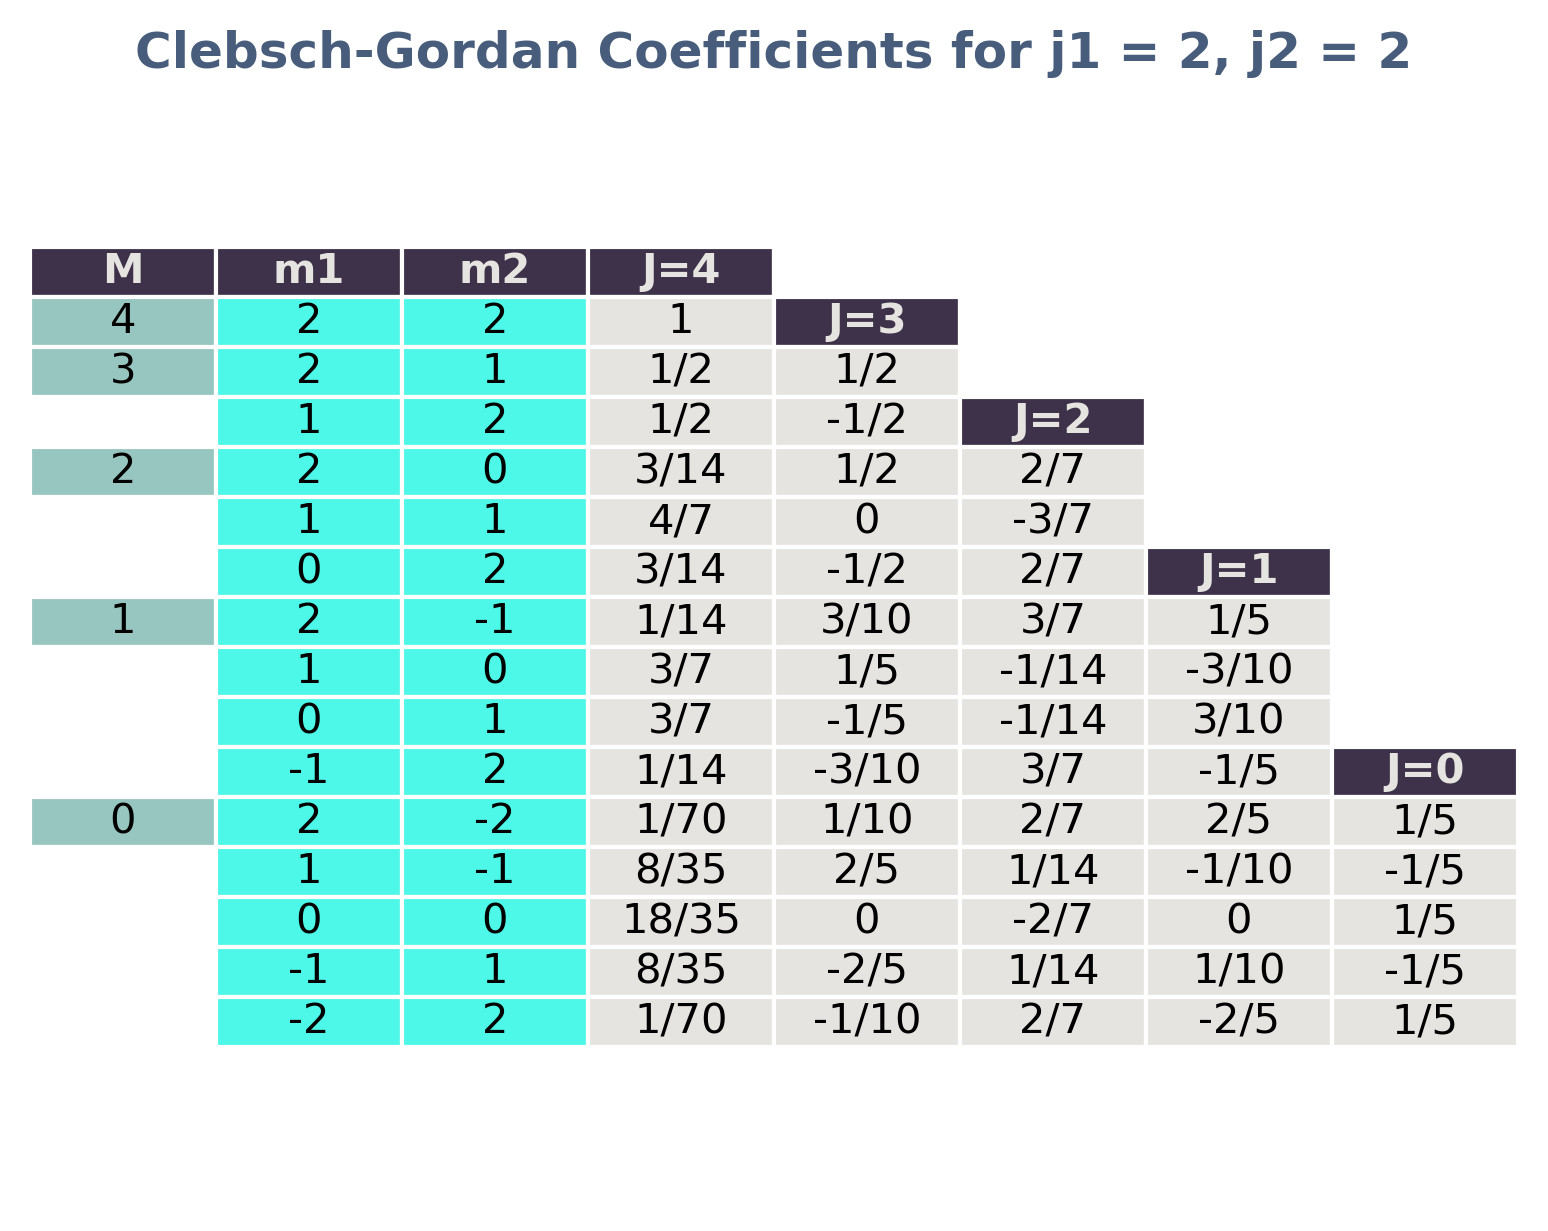
\includegraphics[width=\linewidth]{images/cgc_example}
	\caption{利用代码绘制的CG系数表}
	\label{fig:cgcexample}
\end{figure}



%---------------------------------------------------------------------
% 参考文献
\clearpage
\ysySection{参考文献}

% 编号、作者、文章名、文章类型、期刊名、发表时间和卷(期):页
\begin{enumerate}[label=\textbf{[\arabic*]},ref=\arabic*]
	\ysyRef{a}{Einstein, A., Bohr, N.}{A Remarkable Paper About Quantum Theory}{J}{Physical Review}{1925}{1(4): 1-111}
	\ysyRef{b}{Wikipedia contributors}{Lock-in amplifier}{EB/OL}{Wikipedia, The Free Encyclopedia}{2025}{\url{https://en.wikipedia.org/wiki/Lock-in_amplifier}}
\end{enumerate}

格式如下：
\begin{table}[h!]
	\resizebox{\textwidth}{!}{\begin{tabular}{|l|l|p{8cm}|}
		\hline
		\textbf{项目} & \textbf{示例} & \textbf{说明} \\
		\hline
		作者 & Einstein, A., Bohr, N. & 英文作者名不必翻译，多个作者用逗号隔开 \\
		\hline
		题名 & A Remarkable Paper About Quantum Theory & 原标题，英文标题首字母大写 \\
		\hline
		文献类型 & [J] & 表示期刊论文 \\
		\hline
		期刊名 & Physical Review & 期刊名（可斜体，视期刊要求） \\
		\hline
		年份 & 1925 & 出版年份 \\
		\hline
		卷号 & 1 & 卷 \\
		\hline
		期号 & (4) & 期 \\
		\hline
		页码 & 1-111 & 页码范围 \\
		\hline
	\end{tabular}
}
\end{table}


引用\cref{ref:a}和\cref{ref:b}。